%%% template.tex
%%%
%%% This LaTeX source document can be used as the basis for your technical
%%% paper or abstract.

%%% The parameter to the ``documentclass'' command is very important.
%%% - use ``review'' for content submitted for review.
%%% - use ``preprint'' for accepted content you are making available.
%%% - use ``tog'' for technical papers accepted to the TOG journal and
%%%   for presentation at the SIGGRAPH or SIGGRAPH Asia conference.
%%% - use ``conference'' for final content accepted to a sponsored event
%%%   (hint: If you don't know, you should use ``conference.'')

\documentclass[review]{acmsiggraph}
\usepackage{fixltx2e}
%%% Make the ``BibTeX'' word pretty...

%%% Used by the ``review'' variation; the online ID will be printed on 
%%% every page of the content.

\TOGonlineid{paper1040}

%%% Used by the ``preprint'' variation.

\TOGvolume{0}
\TOGnumber{0}

\title{SVGPU: Real Time 3D Rendering to Vector Graphics Formats}

\author{Apollo I. Ellis and Warren Hunt and John C. Hart}
\pdfauthor{Stephen N. Spencer}

\keywords{3d, vector graphics,real time rendering, GPU}

\begin{document}

%%% This is the ``teaser'' command, which puts an figure, centered, below 
%%% the title and author information, and above the body of the content.

 \teaser{
%    \includegraphics[height=1.5in]{images/sampleteaser}
%   \caption{Spring Training 2009, Peoria, AZ.}
 }

\maketitle

\begin{abstract}

Rendering realistic 3D scenes to vector graphics in real time may have been a
hot topic decades ago, but has now again become interesting, as display
resolutions grow rapidly and resolution independent rendering supports display
across a wide variety of devices. Further in the advent of cloud gaming raster
images for large displays will prove a significant bottleneck when being
transported over networks from server to client. We implement a real time
rendering pipeline that utilizes a novel analytic visibility algorithms to
output a compact vector graphics representation of a 3D scene. Our system is
fast and efficient on modern hardware and thus enables the benefits vector
graphics representations to reaped by the real time community.

\end{abstract}

\begin{CRcatlist}
  \CRcat{I.3.7}{Computer Graphics}{Three-Dimensional Graphics and Realism}{Hidden line/surface removal}
  \CRcat{I.3.7}{Computer Graphics}{Three-Dimensional Graphics and Realism}{Visible line/surface algorithms};
\end{CRcatlist}

\keywordlist

%% Required for all content. 

\copyrightspace

\section{Introduction}
In the earliest days of computer graphics, the VRAM needed for a raster
framebuffer was prohibitively expensive, and graphics was output in a vector
format. Hidden line algorithms were needed to convert 3-D scene geometry into
a planar map of view projected regions with depth complexity one, so their
outlines could be displayed on the vector display devices available then. Even
though raster displays have been available for decades, the output of 3-D
scenes as a vector planar map is still a valuable process for many
applications. For example, the real-time rendering of 3-D shape outlines was a
primary feature behind the appeal of the Teddy sketch-based modeling interface
\cite{igarashi1999}.

As the output of a 3-D scene renderer, a planar map image of 2-D polygons has
several advantages over a raster image of pixels. First, vector images provide
a resolution independent representation that can be efficiently rasterized at
any resolution onto an arbitrarily sized display, ranging from watches to
videowalls to head-mounted displays. The rasterization of a planar map consists
of point-in-polygon
tests and avoids the need to sort depth, and so does not suffer the
pathological issues of depth buffering, c.f. \cite{lapidous1999}. Moreover, the
planar map vector image allows rasterization to be delayed until display, so
the display's resolution can be accomodated, and proper edge antialising can be
performed, e.g. \cite{manson2011}.

\begin{figure}[t] \centering
\includegraphics[height=3in]{images/bunny-red.png}
\caption{A toon shaded Stanford bunny of 70K triangles rendered as a
resolution-independent planar map of visible triangle portions (depth
complexity is no greater than one) in about 30 ms (33 Hz) by the SVGPU vector
renderer, representing a three-fold improvement over previous GPU vector
renderers.}
\end{figure}

Second, in an era where wireless network bandwidth is a critically
valuable commodity, vector images are compact, reducing both network
consumption and latency. Cloud gaming is an emerging trend of the video gaming
industry, where the display image of a video game is rendered by a server and
transmitted over the internet to a thin client. Current gaming-as-a-service
(GaaS) systems render raster images that are transmitted as MPEG streams, but
these streams consist of full resolution I-frames because the computation of
block motion on these raw images needed for more efficient MPEG transmission
creates too much latency. A server rendering 3-D game scenes directly to a
planar map yields correspondences that would better support motion for more
efficient game video transmission.

The computation of analytic visibility was recently shown to be practical on
the GPU with an edge-based renderer \cite{auzinger2013}. They
showed that analytic visibility could be computed faster than the
multisampling needed to properly rasterize some pathological cases.

In this paper we present a real-time triangle-based vector renderer that
converts a 3-D meshed scene into a planar map of 2-D triangles. This result can
be directly converted into a vector graphics representation (e.g. SVG)
or can be quickly rasterized without need for a depth buffer and with
display-resolution-dependent edge antialiasing \cite{reshetov2009,jimenez2012}.
This system also extracts the visual contour as well as the regions it bounds,
and both can be easily stylized for non-photorealistic rendering.

\begin{figure*}
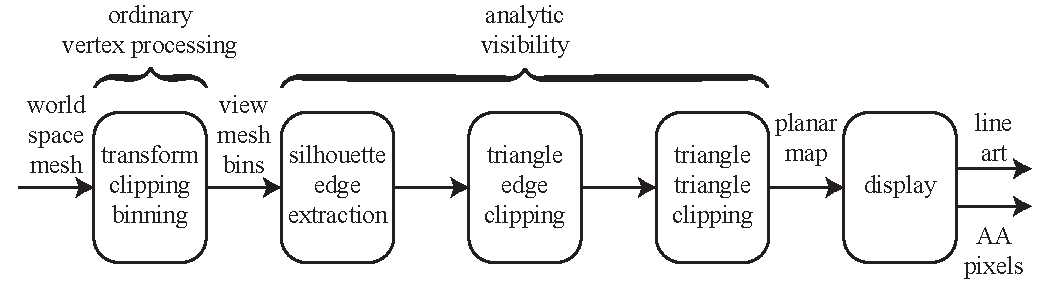
\includegraphics{images/pipeline.pdf}
\caption{The stages of our binned vector graphics rendering system.}
\label{fig:pipeline}
\end{figure*}

Our pipeline consists of five stages described in Section~\ref{sec:svgpu}. The
first stage performs transform,
clipping, and binning operations, which is borrowed directly from the
rasterization pipeline, and we make no noteworthy additions to these
operations. The next three stages form the main contribution of the analytic
visibility pipeline. The second stage, described in
Section~\ref{sec:silhouette} performs silhouette extraction using GPU
spatial hashing to quickly find neighboring frontfacing-backfacing triangle
pairs with a linear sweep through the mesh. The third stage described in
Section~\ref{sec:clipping} clips triangles to
the extracted silhouette edges, limited to the geometry in each bin, using
dynamic parallelism to better balance load across bins representing
different amounts of geometry. This silhouette clipping of triangles allows
the fourth stage described in Section~\ref{sec:occlusion} to simply cull
triangles if any occlusion is detected, which
is a quadratic-time comparison between all-pairs of triangles in a bin.
The fifth stage our system outputs the result, either as a vector
representation of the planar map of triangular regions, or by rasterization of
the depth-complexity-one, which provides additional benefits for edge
antialiasing and resolves some depth rendering issues.

The design of our vector renderer is based on the idea that we use the same
spatial coherence and streamed processing tricks developed for fast
rasterization graphics pipelines to accelerate the rendering of vector
graphics. These tricks include binned rendering and spatial hashing, as well
as load balancing and tuning, which is analyzed in Section~\ref{sec:results}

% The visibility pipeline must feature every visible surface, there should be no
% overlap, and it must output geometry which can be rendered to produce a scene
% faithful to one rasterized with vertex attribute interpolation. The hidden
% surface element is solved in our system by a sequence of categorization and
% clipping operations. The clipping operations in turn satisfy the no overlapping
% condition [TODO:rephrase]. Since the visibility operations remove all hidden
% elements accurately (analytically) and leaves all visible geometry, we
% faithfully represent the scene in 2D. This planer map may be rasterized
% without condideration for depth in such a way that it is indistinguishable
% from an image produced by a traditional raster pipeline.  This analytic
% pipeline has complexity on the order of the geometry, rather than the order of
% the resolution of the final image and becomes relatively more efficient as
% final render target resolution increases.

\section{Previous Work}
The hidden line problem was well studied decades ago \cite{sutherland1974}.
Most modern approaches been based on Appel's algorithm \cite{appel1967} which
extracts continuous silhouette components to display, computing the
quantitative invisibility as these components cross each other.
The main benefit of Appel's algorithm is that once the silhouette is
extracted (after a linear pass through the scene polygons), the polygons no
longer need to be processed, and comparisons only need to occur along the
silhouette edges, significantly reducing computation. The main drawback is
that the mesh silhouette is plagued with special cases, including cusps,
switchbacks and non-transverse intersections that can affect robustness. Our
approach clips triangles instead of the silhouette to the silhouette edges,
and does not require the silhouette edges to be connected into a continuous
curve for fragile incremental visibility computation.

Robert's algorithm is an even older approach that simply compares all pairs of
scene polygons, clipping and culling occluded portions of polygons
\cite{roberts1963}. These all-pairs comparisons were slightly reduced 
using bounding boxes, but still resulted in a quadratic time complexity, but
also a significantly more robust output than Appel's algorithm. Our SVGPU
approach leverages this robustness, and further reduces the impact of
quadratic all-pairs triangle occlusion comparisons through binning, in
addition to other culling strategies, and maps better to the brute force
streaming parallelism offered by modern GPU's than does Appel's algorithm.

A large number of non-photorealistic rendering systems have included renderers
that convert a 3-D scene into 2-D planar map
\cite{winkenbach94,hertzmann2000,stroila2008,eisemann2008,eisemann2009,karsch2011},
but these have largely been offline CPU programs that focused on the quality
of the output. Some have looked at the real-time NPR, e.g. by fast (sublinear)
statistical gloabl searches for seed segments of the silhuette
\cite{markosian1997}, instead of our linear-time spatial hash approach to
silhouette extraction. A variety of other techniques have also been employed
to accelerate NPR rendering based on actual silhouette edges
\cite{buchanan2000,kim2005} or their approximation \cite{raskar1999}.
Some have also developed hardware solutions for real-time NPR contour
extraction \cite{raskar2001,ho2004,wang2005}.

The GPU has been used to compute the high-quality visibility of stylized lines
by using a texture atlas as an intermediate frame buffer for compositing
\cite{cole2009}, but the actual visibility is based here on the depth buffer.
The GPU was also used for analytic visibility of polygons, using an edge-based
approach \cite{auzinger2013}, whereas out approach is triangle based, using
the silhouette edges only for clipping to yield better performance results.


% \item RYU, D. 2001. Visibility Layer Decomposition. Senior thesis, Harvard University.
%  Ryu seems to have been modernized by Eisemann 2009 so no need to cite now

% \item AUZINGER T., GUTHE M., JESCHKE S.: Analytic Anti-Aliasing of Linear Functions on Polytopes.
% Nah

\section{The SVGPU Pipeline} \label{sec:svgpu}

The input to our pipeline is a 3-D scene consisting of triangle meshes,
represented as an indexed face set, without need of an edge-based data
structure, and in fact our approach works with triangle soup. We do not require
the meshes to be manifold but non-manifold edges and boundary edges will be
classified as silhouette edges.  We do require that no triangle pierces any
another triangle, which simplifies clipping and occlusion.

The first stage of our pipeline performs the ordinary vertex processing
pipeline found in common rasterization systems, such as OpenGL. This stage
transforms world-space triangles into a perspective viewed ``window''
coordinate system.  The triangles are then organized and clipped into 2-D grid
of viewing bins organized across the window.

\subsection{Silhouette Extraction} \label{sec:silhouette}
SVGPU uses a spatial hash table, which can be efficiently constructed and
accesssed on the GPU \cite{lefebvre2006}, to detect which edges form the
silhouette. (We use the term silhouette in this paper loosely, to refer to the
visual contour of edges shared by both frontfacing and backfacing triangles.)
For each of the three edges of
every triangle, we sort its two vertices by their 3-D coordinates, and use
these sorted 3-D coordinates to create a hash key. We then add the triangle to
the hash table at three places corresponding to the hash keys of its three
edges. Once all triangles have been entered into the hash table, the silhouette
edges are extracted as entries whose normals (in projected viewing coordinates)
have oppositely signed $z$ values. We also include as silhouettes any edges
where the hash table lists any number of triangles besides two.

% hash based approach is employed which is easy to implement, can be parallelized on GPUs, and provides the analytically correct silhouette edges. The hash key is based on the indices from the indexed face set in pairs of two per edge. Note that spatial hashing would also work in the case where the input is triangle soup, but an index face set in used in the experiments in this paper. The hashing stage requires hash key computation, silhouette edge detection on hash collision, and hash table writes.

% First a hash key must be computed for each edge and then hashed to detect silhouette edges. For each pair of two 32 bit indices the bits are interleaved and the result is moded by a large prime number [TODO:why do we mod by a large prime?]. If the two indices were instead appended together the hash location would largely depend only on the lower order index which may produce a bad hash function. So interleaving is used. The next step is to check if there are other edges in the hash location and if so compare the z values of the normal associated with two triangles sharing an edge. If the normal vectors are a positive-negative pair this edge is marked as a silhouette. Otherwise the edge data is written into the hash table bucket at that key’s location. 

% As previously stated computing silhouettes is important to our pipeline because it simplifies the clipping computations needed to compute analytic visibility. Silhouettes have additional benefits to rendering, as previously mentioned. Silhouette processing simplifies the computation in two ways. Now the system only needs to compute the clipping of each triangle against one edge at a time, the silhouette edges. Alternatively it would be necessary to compute a full triangle vs triangle clip or clip multiple edges against multiple edges as in previous approaches. Secondly, each triangle has already been clipped against all possible silhouette edges so there is no need to perform a full clip in the next stage. It becomes sufficient to check if a triangle begins to clip or “would clip” another triangle. If this is the case it’s ok to discard the other triangle because if one triangle partially occludes another that triangle must be a silhouette edge and those cases are handled first.

\subsection{Clipping} \label{sec:clipping}
%	In this stage the goal is to clip every triangle in a bin to the all the silhouette edges in that bin. The act of actually clipping a triangle to a silhouette edge occurs much less frequently than the act of discounting the need to clip a triangle against any of the silhouette edges. Further since clipping a triangle to a silhouette edge may produce new triangles that would then also need to be clipped by edges, this stage has been segmented to retain instruction execution coherence on GPUs.

This stage clips every triangle in a bin to every silhouette in the bin. Since
we expect the number of triangles that overlap each silhoette edge to be
small, we segment this stage into two steps: a culling step and a clipping
step, to retain GPU instruction coherence.

% The culling step is used to remove most triangle-edge pairings from
% consideration for clipping. This step consist of three tests.
% \begin{enumerate}
% \item If the window projection of all three triangle vertices lie on one side
% of the window projection of line passing through silhouette edge, then cull.
% \item Compute $z$ coordinates of the points on the triangle and the
% line passing through the silhouette edge where the window projection of the
% triangle edges cross the window projection of the line passing through the
% silhouette edge. If the silhouette edge is behind the triangle, then cull.
% \item If neither of the intersection points on the line passing through the
% silhouette edge lie on the silhouette edge itself, and the silhouette edge
% does not lie between these points on the line, then cull.
% \end{enumerate}

The culling step is used to remove most triangle-edge pairings from
consideration for clipping.
Let $(x_1,y_1,z_1), (x_2,y_2,z_2)$ and $(x_3,y_3,z_3)$ be the window
coordinates of a triangle $\Delta 123$, and let $(x_A,y_A,z_A)$ and
$(x_B,y_B,z_B)$ be the window coordinates of the silhouette edge
$\overline{AB}$. Then this culling step consist of three tests.
\begin{enumerate}
\item If $(x_1,y_1), (x_2,y_2)$ and $(x_3,y_3)$ lie on one side of the line
passing through $(x_A,y_A)$ and $(x_B,y_B),$ then cull.
\item Let $C$ and $D$ be the points on the line passing through $A$ and $B,$
and let $4$ and $5$ be the points on the edges of $\Delta 123,$ such that
$(x_C,y_C) = (x_4,y_4)$ and $(x_D,y_D) = (x_5,y_5)$ indicate where the
window projection of the silhouette edge crosses the window projection of the
triangle. If $z_C$ and $z_D$ are behind (less than) $z_4$ and $z_5,$ then cull.
\item If $\overline{CD} \cap \overline{AB} = \emptyset,$ then cull.
\end{enumerate}

We also cull if (4) the silhouette edge is an edge of the triangle, (5) if the
triangle is back facing, and (6) if the triange is obviously in front of the
silhouette edge: $\min z_1,z_2,z_3 > \max z_A,z_B.$

This segment is implemented as an $m \times n$ kernel that considers the
coverage of $m$ triangles by $n$ silhouette edges, so each thread considers
if one specific triangle covered by one specific silhouette edge. If the
thread survives all three culling tests, then it outputs the triangle and
silhouette edge ID's to a list for processing by the next segment of this
stage.

% To check for clipping three tests are employed. The first is a point on edge side test. If the test returns a non-trivial result, i.e. different vertices fall on both sides of the edge the stage proceeds, otherwise it returns. Proceeding is to compute the intersection points at which triangle crosses the silhouette edge. The z values of these points are then checked against the z values of the corresponding xy locations on the silhouette edge’s triangle plane and the algorithm returns if these intersection points are in front of the plane. Lastly it is necessary to check if the intersection points lie either inside the silhouette edge interval or on opposite sides. The second case accounts for a silhouette edge which lies completely inside a partially occluded triangle. If neither occurs the algorithm returns, but if it did not return early the triangle is marked as needing to be clipped by the second segment of this stage.

The first segment yields the list of pairings of silhouette edges that cross
triangles in the bin. For each bin, we organize these pairings into a table of
triangles, such that for each triangle in this table, there is a corresponding
list of the silhouette edges that clip it. The second segment of this stage
will subdivide each triangle by each of its corresponding silhouette edges
that cover it, producing as many as three triangles. We cannot remove any of
these three sub-triangles as they may be further clipped by other silhouette
edges.  If a subtriangle would be hidden by one silhouette edge, a
portion of it may be revealed by a subsequent silhouette edge.

% In the second segment a full and triangle vs edge clipping must occur, which may generate new geometry. The new geometry may require additional clipping. Essentially there may exist a triangle that is clipped by an edge and then in turn the new geometry is clipped by other silhouette edges. This requires care in parallelization to handle load balance but our algorithm is fairly straightforward [TODO: straitforward? does it achieve load balance?].

% To clip a triangle against an edge is as follows. First it must be determined which edges overlap the silhouette edge. In the case where the two edges overlapping are extending from one vertex, the algorithm clips off the un-occluded triangle region, divides the remaining region in two triangles, and writes all three back into a buffer for further clipping by other edges. In the case where the two edges are extending from two different vertices the inverse operation occurs, clipping off a two triangle quad, and writing back these and the left over triangle to a buffer for further processing. The algorithm is simple and can be implemented efficiently on a GPU. However, again, the GPU implementation will take some care in design to avoid load imbalance.

Due to the varying number of new sub-triangles that can be generated when
triangles are clipped, this second segment can easily suffer a load imbalance.
To balance the workload evenly, we employ a work queue method based on dynamic
parallelism, as available e.g. from NVidia's Compute model 3.5+ GPU's. In this
approach, kernels are launched in rounds, and each round can determine how many
threads to generate in the next round based on the work generated.

The first round assigns one thread per triangle in each bin, and each of these
threads begins by clipping the triangle to one of the overlapping silhouette
edges. If this creates three triangles, then those three triangles are added to
the thread queue for the next round which processes the next silhouette edge
in each triangle's list. These rounds are double buffered, such that each
round reads the triangle data from one buffer and writes the subdivided
triangles to the other buffer, which will be the input for the next round.

\subsection{Occlusion} \label{sec:occlusion}

Since all of the triangles have been clipped to silhouette edges by the
previous stage, and since there are no piercing triangles, then each remaining
triangle is either entirely visible (part of the planar map) or occluded and
can be culled.

The occlusion phase compares all pairs of (clipped) triangles in the bin. We
launch one thread for every pair of triangles to determine if one occludes the
other. This yeild a large number of threads and is very sensitive to the
choice of bin size as it related to the number of triangles in a bin.


% The last phase of our visibility infrastructure consists of checking triangles for occlusion by other triangles. This check is a simplified version of triangle-triangle clipping. A similar method as in the first segment of triangle vs silhouette edge clipping is used here. The only information needed is whether a triangle would need to clip a given triangle, in fact the tests are exactly the same as before. The triangle id is written to a visible list if the algorithm did not return early (e.g. because it would have needed to clip).

% \section{Implementation}
% We implement our pipeline primarily on the GPU using Cuda kernels with some CPU orchestration. Vertex shading and clipping are separate kernels. One kernel computes model view projected vertices, and the next assembles triangles checks if they need be to clipped to z cross 0 plane. If clipping is needed then any newly generated clip geometry is written into a buffer for binning and divide by w also occurs in this kernel. Now the triangles must be binned by bounding box. Triangle vertex data is stored in the bins along with id, simplifying the kernels in further stages. The binned triangles contain four floats per vertex with indices packed into w, and a face normal.
% \subsection{Silhouette Hashing}
% The implementation here is straightforward GPU based hashing over the entire input set. Since the complexity of this operation is somewhat independent of bin size, all edges in the screen are hashed in the same kernel. An m by n kernel is launched where n is the number of bins and m is the total triangle count divided by n. Each column of threads in the grid is reading from one bin.

% Our kernel calculates hash keys by interleaving the index bits, hashes edges, and marks silhouettes. An edge is not always written into the hash table, the write requires GPU atomics to increment counters for the hash buckets associated with the keys. Better to not do an atomic if not necessary, so the write happens only after checking hash table contents for adjacent edges. If the edge’s pair is not available it will have to be written and read back by a different thread [TODO: is there a race-condition here?]. If it is available the z values are compared and if they are oppositely signed it is marked. To mark a silhouette edge the kernel writes its id into a buffer location indexed by an atomic counter. 

% This leaves the problem of marking unmatched edges as silhouettes, so during hashing a flag is set on the hash table every time a location gets an edge, de-asserting when an edge pair is found, and re-asserting when another edge arrives. After the kernel returns a cleanup kernel writes back any edges left behind. NVidia’s compute model 3.5+ dynamic parallelism is used here but the discussion is left for the next section where its usage is more critical to our implementation.


% \subsection{Triangle vs Edge Clipping on the GPU}
% As mentioned the triangle vs edge clipping phase is cut into two segments, a categorization segment, and a clipping segment. In the first segment an m by n kernel is launched to the GPU to clip m triangles against n edges. Each thread m\textsubscript{i}n\textsubscript{j} is responsible for determining whether a triangle  m\textsubscript{i} is clipped by edge n\textsubscript{j}. If this is the case the kernel writes out the triangle id to a list for further processing. As mentioned in the algorithm section if this is not the case the thread retires. This kernel is simple, but the kernel that follows is much more complex due to a load balancing problem.

% In the second segment triangle vs edge clipping operations occur which can generate additional operations. To balance the work on the GPU a work queue method based on dynamic parallelism is used. Dynamic parallelism, available on Nvidia’s compute model 3.5+ GPUs, affords us the ability to launch a kernel from within a kernel to avoid expensive CPU-GPU synchronization, data transfers, and driver overhead. Kernels are launched in rounds where each round determines how many threads to enque to the next round based on the work generated.

% The first kernel clips all triangles from each bin that contained silhouettes with a single silhouette edge from each bin. Recall that as a triangle is clipped against an edge it generates one or two new triangles and writes them to storage. If there are more edges in a bin a kernel always enques three threads to the next round kernel, one for each clipped triangle region. Care is taken to write the new triangles back to a location index-able in the next phase by the so called child threads of the current phase. In that next phase each child thread reads its triangle based on its newly generated thread id and the next edge to process is accessed from a list via an atomic counter. The deeper details of the id based look up scheme are beyond the scope here, but the interested reader is encouraged to refer to Nvidia’s Cuda Compute API 3.5+ for more on dynamic parallelism. 

% \subsection{Occlusion Pass}
% This phase operates in a single kernel and reuses code from the triangle vs edge clipping section. If it is determined that there would be need to clip a triangle is it discarded. The kernel is m by m by n grid where m is the number of triangles in a bin and n is bin count. For reference the bin size used is 128x128 pixels. While this phase is simple it is also fast, a byproduct of the main contribution of our silhouette based algorithm, simplified clipping.

% \subsection{Rendering}
% At this point in the pipeline there two options, render directly, or send to a client. Our rendering implementation invokes OpenGL with the depth buffer disabled and uses a pass through vertex shader. Phong shading is implemented in the pixel shader. It follows from this that the system has met the goal of representing the scene as a planar map since it OpenGL can effectively render our output directly. To further show validity as a vector graphics format a rendering backend that uses the Nvidia’s path rendering API is also in place.

\section{Results} \label{sec:results}
Our prototype implementation is demonstrated on a variety of well known models,
specifically the bunny, armadillo, dragon and buddha. Each of these models was
represented as an indexed face set, and for these examples our silhouette
extraction used a hash on the vertex indices instead of the vertex
coordinates, which was inconsequential as silhouette hashing was less than a
millisecond for all of these examples.

\begin{table*} \centering
\begin{tabular}{|l|c|c|c|c|c|c|c|c|} \hline
\bf Model & \bf $\Delta$ in & \bf $\Delta$ out & \bf bin size & \bf nonempty
bins & \bf max $\Delta/$bin & \bf ave. $\Delta/$bin & \bf time (ms) \\
\hline
Bunny & 69K & 280K & $1/48^2$ & 754 & 698 & 139 & 41 \\ 
Dragon & 202K & 950K & $1/48^2$ & 444 & 1,740 & 555 & 222 \\
Armadillo & 212K & 1.2M & $1/(48\times 24)$ & 509 & 2,076 & 356 & 256 \\
Buddha & 293K & 1M & $1/48^2$ & 985 & 712 & 200 & 140 \\ \hline
\end{tabular}
\caption{Rendering performance on various models.}
\label{tab:modelperf}
\end{table*}

Table~\ref{tab:modelperf} compares the performane of the SVGPU renderer
across several models. The Dragon and Armadillo models are about $3\times$ the
size of the bunny, but require roughly $6\times$ as much time to render,
indicating some impact of the quadratic all-pairs triangle occlusion step. The
tiled approach, combined with aggressive parallelism helps to avoid the
$9\times$ render time that would be expected when a quadratic step dominates
the process. The Buddha model contains even more geometry, but includes larger
triangles and is distributed across more tiles, and so renders in
significantly less time.

\begin{figure} \centering
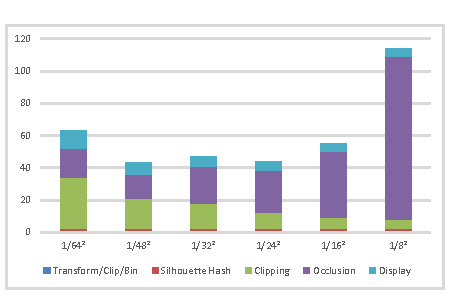
\includegraphics{images/binperf.pdf}
\caption{Performance (ms) of tiled vector rendering of the Stanford bunny mesh,
for tiles sizes ranging from $1/64^2$ of the window (4,096 tiles) to $1/8^2$ of
the window (64 tiles).}
\label{fig:binperf}
\end{figure}

Figure~\ref{fig:binperf} analyzes the performance of the SVGPU binned vector
renderer across different bin sizes. As bins grow larger, from $1/64^2$ to
$1/8^2$ of the window, the time spent on clipping decreases while the time
spent on occlusion grows quickly. Since the occlusion stage performs an
all-pairs comparison of the triangles in each bin, it is quite obvious that
smaller bins will contain fewer triangles which will reduce the number of
comparisons quadratically. However, smaller bins results in more bins, and
greater variation of the numbers of triangles in a bin, which hinders the load
balancing of the clipping of triangles to silhouette edges implemented using a
dynamic parallelism work scheduler. The best compromise uses a bin size of
$1/48^2$ of the window size, but achieves a decent balance from there to
$1/24^2.$

\subsection{Rebinning}
As Figure~\ref{fig:binperf} reveals, the bin size affects the performance of
the vector renderer. Smaller bin sizes reduce the number of triangles for the
occlusion stage's all-pairs quadratic comparison, whereas larger bin sizes
hold more triangles which supports better load balancing during the clipping
stage.

We have implemented a rebinning solution, such that larger bins are used for
the clipping stage, and these bins are subdivided into smaller bins for better
performance of the occlusion stage. This rebinning stage, between the clipping
and occlusion stages, subdivides the clipping bin into smaller occlusion bins,
clipping the existing triangles output by the clipping stage to the new
smaller occlusion bin boundaries.

Our experiments on the bunny mesh showed that rebinning incurred a 3ms delay,
in our case rebinning $1/8^2$ clipping bins to $1/64^2$ occlusion bins.
However, this rebinning maneuver resulted in an overall improved rendering
rate of 30ms (reduced from the 41ms using fixed bin size), so the additional
3ms rebinning investment saves 14ms in the quadratic occlusion step.

\subsection{Comparison with Previous Work}

Prevous results from analytical visibility on the GPU \cite{auzinger2013}
render the 70K-triangle bunny at a variety of raster resolutions in a time
ranging from 172 to 212 ms, on an NVidia GeForce GTX 680, which has 1,536
cores running at 1GHz. Our results were computed on an NVidia GeForce GTX 980,
which has 2,048 cores running at 1.1GHz. Comparing results from different
GPUs is a complex process, but we can estimate that since GTX 980 represents
33\% more cores running 10\% faster, we should see about a 47\% improvement in
speed over the 680 used for analytical visibility's results (ignoring many
other differences, including e.g. memory bandwidth). The improved rebinning
SVGPU renders the bunny into a planar map at 30ms, whereas analytic visibility
running 47\% faster would render the bunny in about 117 ms, leading us to
believe SVGPU is about three times faster.
 
\section{Conclusion}
% As mentioned we envision a client server model equipped with our system. We imagine this either as a cloud server serving to a low-power machine or, similarly, a powerful machine streaming to a VR HMD. In these model a scene would be submitted to the pipeline server which proceeds to transform, clip, and perform our custom visibility outputting a planar map representation. Then the scene can be sent to the client in its compact form with low latency. The client could avoid all depth-related computation and need only be able to perform point in polygon tests, interpolation, and fragment shading. This hypothetical rasterizer doesn’t even need a z buffer. So it would be consuming almost no bandwidth. [TODO: Not sure I buy this argument.  Due to z-compression, z-buffer bandwidth isn't extreme relative to texture or g-buffer bandwidth used during shading computations]

We have shown that the GPU can implement a vector rendering system suitable
for generation of line art or for rasterization with improved edge
antialiasing and visible surface processing. By binning geometry into small
screen tiles, about $1/48^2$ of the screen size, we achieve an optimal domain
decomposition that distributes a parallel clipping workload evenly while
limiting the impact of an all-pairs quadratic triangle occlusion test. The
result yields about a $3\times$ improvement over the state of the art.

There are a few important limitations of this system. Any shading must be
applied separately, for example as a deferred pixel shader on the rasterized
planar map. The subdivision of triangles due to clipping can preserve
perspective-correct interpolation of texture coordinates and other vertex
attributes to ensure the necessary data is available for proper shading.

The planar map output delivers a planar map consisting only of the visible
portion of the visual contour and the regions it bounds, tesselated by many
small clipped triangles (which could be re-merged into larger regions by the
display stage). The inclusion of cast shadows would be a useful addition to
this system. While the outlines of the cast shadows can be determined by
running the process from the point of view of a light source, the integration
of cast shadow contours into the visual contours of the silhouette can be
tricky and is left as future work.

\bibliographystyle{acmsiggraph}
\bibliography{svgpu}
\end{document}
